\documentclass[12pt]{article}
\usepackage[utf8]{inputenc}
\usepackage{graphicx}
\usepackage{multicol}
\usepackage{listings}
\usepackage{amsmath}
\graphicspath{ {./images/} }
\usepackage{amssymb}
\usepackage[htt]{hyphenat}

\usepackage{hyperref}
\hypersetup{
    colorlinks=true,
    linkcolor=blue,
    filecolor=magenta,      
    urlcolor=cyan,
}

\usepackage{xcolor}

\definecolor{codegreen}{rgb}{0,0.6,0}
\definecolor{codegray}{rgb}{0.5,0.5,0.5}
\definecolor{codepurple}{rgb}{0.58,0,0.82}
\definecolor{backcolour}{rgb}{0.95,0.95,0.92}
\definecolor{codeorange}{rgb}{1,0.64,0}

\lstdefinestyle{mystyle}{
    backgroundcolor=\color{backcolour},   
    commentstyle=\color{codegreen},
    keywordstyle=\color{magenta},
    numberstyle=\tiny\color{codeorange},
    stringstyle=\color{codepurple},
    basicstyle=\ttfamily\footnotesize,
    breakatwhitespace=false,         
    breaklines=true,                 
    captionpos=b,                    
    keepspaces=true,                 
    numbers=left,                    
    numbersep=5pt,                  
    showspaces=false,                
    showstringspaces=false,
    showtabs=false,                  
    tabsize=2
}

\lstset{style=mystyle, breaklines=true, postbreak=\mbox{\textcolor{red}{$\hookrightarrow$}\space}}

\title{\vspace{-1cm}Spectra of Non-Periodic Signals\\
\large Assignment 8\\
\large EE2703 - Applied Programming Lab}
\author{Abhigyan Chattopadhyay \\
EE19B146}
\date{21st May 2021}
\usepackage[margin=0.75in]{geometry}

\begin{document}
\maketitle
\tableofcontents
\pagebreak
\section{The Problem at Hand}
This time we will use the Fourier Transform to find the spectrum of various signals which use the same structure as the previous assignment.

\section{Question 1 - Solving through the Examples}

\subsection{Example 1 - Periodic Waveform}

\begin{lstlisting}[language=python]
t=np.linspace(-np.pi,np.pi,65)[:-1]
fmax=1/(t[1]-t[0])
y=np.sin(t)
y[0]=0 # the sample corresponding to -tmax should be set zero
y=np.fft.fftshift(y) # make y start with y(t=0)
Y=np.fft.fftshift(np.fft.fft(y))/64.0
w=np.linspace(-np.pi*fmax,np.pi*fmax,65)[:-1]
plot_spectrum(w,Y,ctr,r"$\sin\left(t\right)$")
ctr+=1
\end{lstlisting}

\begin{center}
    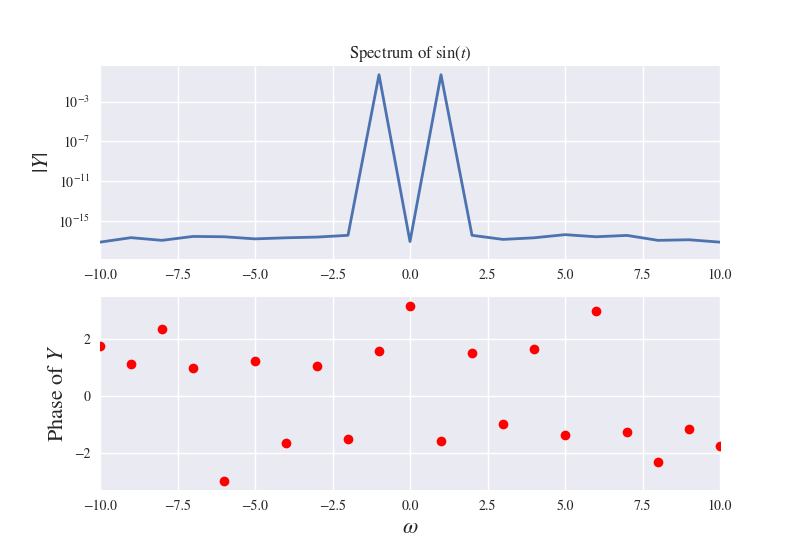
\includegraphics[scale=0.8]{images/fig1.png}
\end{center}
\pagebreak
\subsection{Example 2 - Non-Periodic Waveform}

Here, the wave is not exactly non-periodic, only its frequency can't be expressed as a whole or rational multiple of $\pi$ and hence it appears non-periodic, which we will explore soon:

\begin{lstlisting}[language=python]
y=(np.sin(np.sqrt(2)*t))
y[0]=0
y=np.fft.fftshift(y)
Y=np.fft.fftshift(np.fft.fft(y))/64.0
plot_spectrum(w,Y,ctr,r"$\sin\left(\sqrt{2}t\right)}$")
ctr+=1
\end{lstlisting}

\begin{center}
    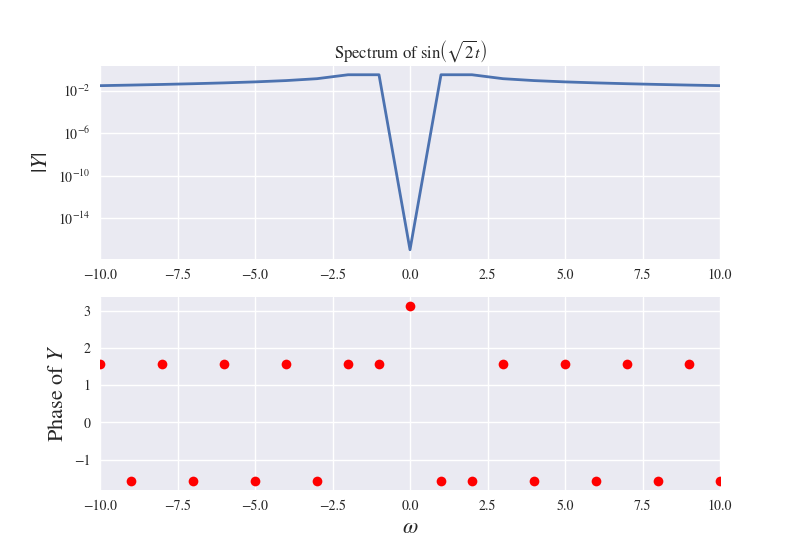
\includegraphics[scale=0.8]{images/fig2.png}
\end{center}
\pagebreak
\subsection{Example 3 - Explaining the Non-Periodic Waveform}
Here we see that the apparent non-periodicity is due to the Gibbs phenomenon at a jump discontinuity due to the sampling of the function over multiple periods.

\begin{lstlisting}[language=python]
t1=np.copy(t)
t2=np.linspace(-3*np.pi,-np.pi,65)[:-1]
t3=np.linspace(np.pi,3*np.pi,65)[:-1]
# y=sin(sqrt(2)*t)
plot_func([t1,t2,t3],[np.sin(np.sqrt(2)*t1),np.sin(np.sqrt(2)*t2),np.sin(np.sqrt(2)*t3)],ctr,r"$\sin\left(\sqrt{2}t\right)$")
ctr+=1

y=np.sin(np.sqrt(2)*t1)
plot_func([t1,t2,t3],[y,y,y],ctr,r"$\sin\left(\sqrt{2}t\right)$ with $t$ wrapping every $2\pi$",marker='o')
ctr+=1

plt.figure(ctr)
plt.semilogx(abs(w),20*np.log10(abs(Y)),lw=2)
plt.xlim([1,10])
plt.ylim([-20,0])
plt.xticks([1,2,5,10],["1","2","5","10"],size=16)
plt.ylabel(r"$|Y|$ (dB)",size=16)
plt.title(r"Spectrum of a digital ramp")
plt.xlabel(r"$\omega$",size=16)
plt.grid(True)
plt.savefig(f"images/fig{ctr}.png")
plt.show()
ctr+=1
\end{lstlisting}

\begin{center}
    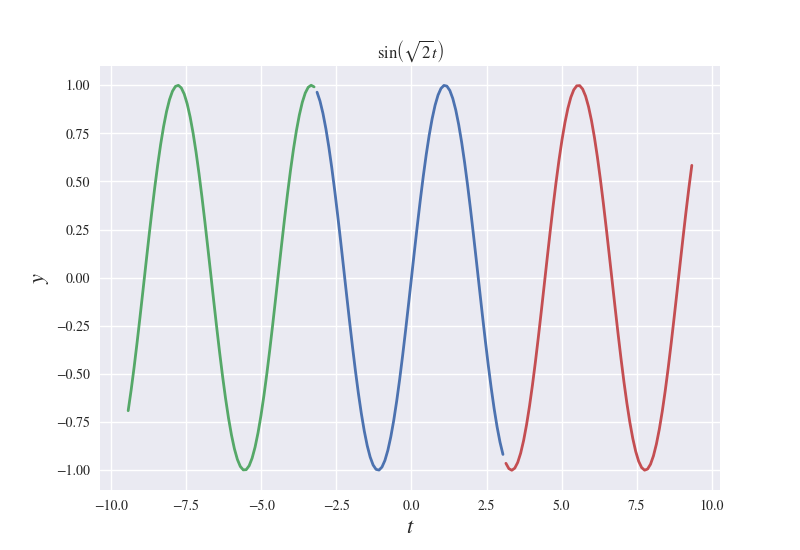
\includegraphics[scale=0.8]{images/fig3.png}
    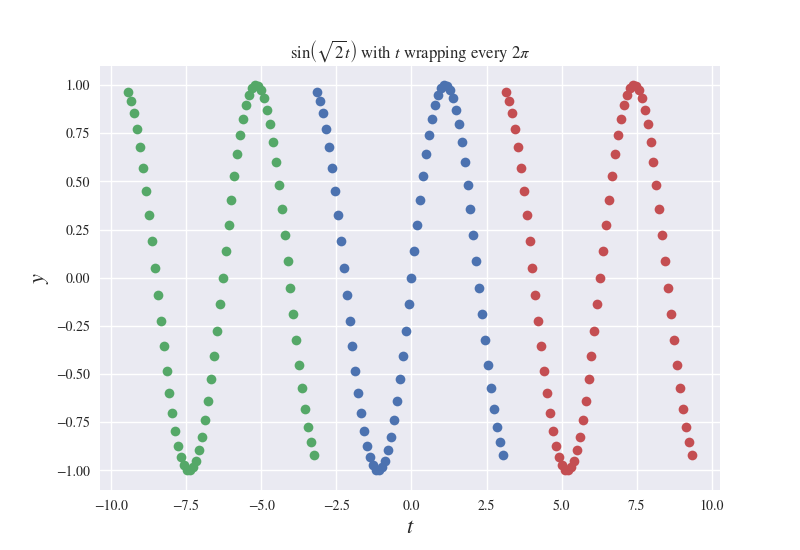
\includegraphics[scale=0.8]{images/fig4.png}
    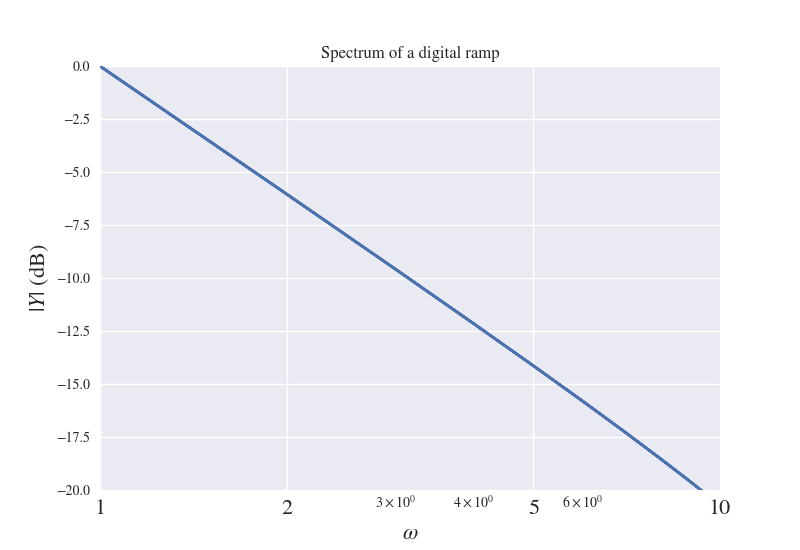
\includegraphics[scale=0.8]{images/fig5.png}
\end{center}

\subsection{Example 4 - Windowing}

Now we use the Hamming Window to generate a better function with a smaller jump.

\[ \begin{cases}
0.54 + 0.46$\cos\left(\frac{2\pi n}{N-1}\right)$ & |n| \leq \frac{N-1}{2} \\
0 & \text{otherwise}

\end{cases}
\]

The jump is still there, but much smaller. It helps by giving us an extra 10dB of suppression.

\begin{lstlisting}[language=Python]
n=np.arange(64)
wnd=np.fft.fftshift(0.54+0.46*np.cos(2*np.pi*n/63))
y=np.sin(np.sqrt(2)*t1)*wnd
plot_func([t1,t2,t3],[y,y,y],ctr,r"$\sin\left(\sqrt{2}t\right)\times w(t)$ with $t$ wrapping every $2\pi$",marker='o')
ctr+=1
\end{lstlisting}

\begin{center}
    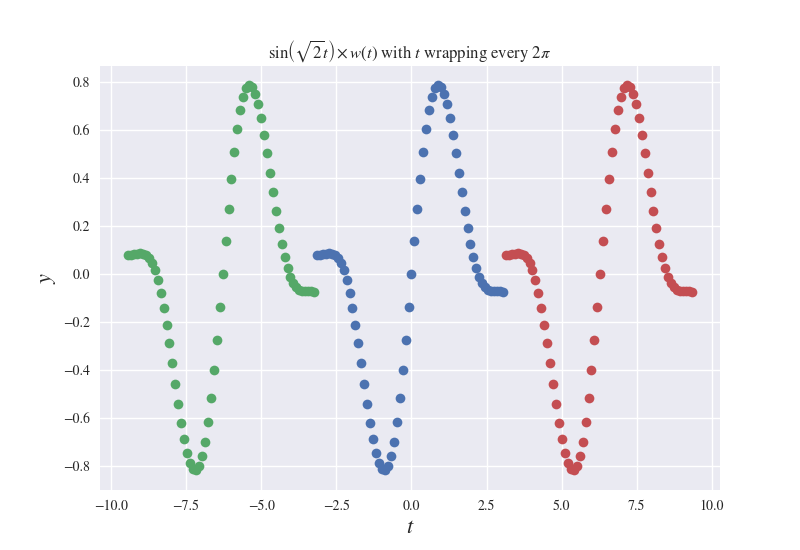
\includegraphics[scale=0.8]{images/fig6.png}
\end{center}

\pagebreak
\subsection{Example 5 - Spectrum with Windowing}

\begin{lstlisting}[language=Python]
t=np.linspace(-np.pi,np.pi,65)[:-1]
fmax=1/(t[1]-t[0])
n=np.arange(64)
wnd=np.fft.fftshift(0.54+0.46*np.cos(2*np.pi*n/63))
y=np.sin(np.sqrt(2)*t)*wnd
y[0]=0 # the sample corresponding to -tmax should be set zero
y=np.fft.fftshift(y) # make y start with y(t=0)
Y=np.fft.fftshift(np.fft.fft(y))/64.0
w=np.linspace(-np.pi*fmax,np.pi*fmax,65)[:-1]
plot_spectrum(w,Y,ctr,r"$\sin\left(\sqrt{2}t\right)\times w(t)$",type='lin',xlims=[-8,8])
ctr+=1
\end{lstlisting}

\begin{center}
    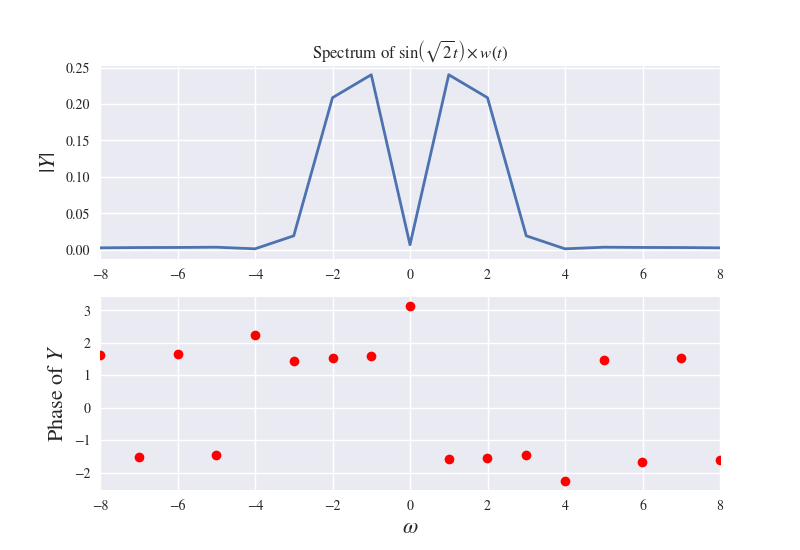
\includegraphics[scale=0.8]{images/fig7.png}
\end{center}
\pagebreak

\subsection{Example 5 - Spectrum with Windowing and More Sampling Points}
\begin{lstlisting}[language=Python]
t=np.linspace(-4*np.pi,4*np.pi,257)[:-1]
fmax=1/(t[1]-t[0])
n=np.arange(256)
wnd=np.fft.fftshift(0.54+0.46*np.cos(2*np.pi*n/256))
y=np.sin(np.sqrt(2)*t)
#y=np.sin(1.25*t)
y=y*wnd
y[0]=0 # the sample corresponding to -tmax should be set zero
y=np.fft.fftshift(y) # make y start with y(t=0)
Y=np.fft.fftshift(np.fft.fft(y))/256.0
w=np.linspace(-np.pi*fmax,np.pi*fmax,257)[:-1]
plot_spectrum(w,Y,ctr,r"$\sin\left(\sqrt{2}t\right)\times w(t)$",type='linpts',xlims=[-4,4])
ctr+=1
\end{lstlisting}

\begin{center}
    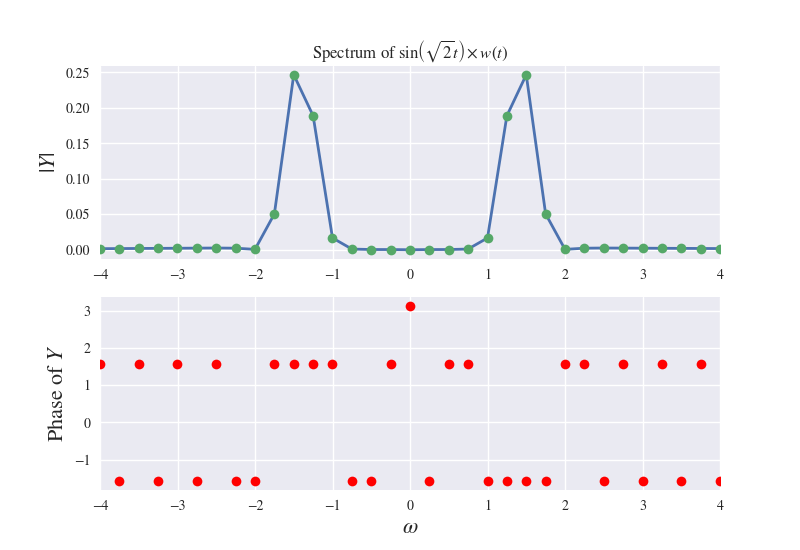
\includegraphics[scale=0.8]{images/fig8.png}
\end{center}
\pagebreak

\section{Question 2 - With and Without Windowing}

$$f(t) = cos^3\left(0.86 t\right)$$

Code:
\begin{lstlisting}[language=Python]
t=np.linspace(-4*np.pi,4*np.pi,257)[:-1]
fmax=1/(t[1]-t[0])
n=np.arange(256)
wnd=np.fft.fftshift(0.54+0.46*np.cos(2*np.pi*n/256))
y1=np.cos(0.86*t)**3
y2=y1*wnd

y1[0]=0 # the sample corresponding to -tmax should be set zero
y2[0]=0 # the sample corresponding to -tmax should be set zero
y1=np.fft.fftshift(y1) # make y start with y(t=0)
y2=np.fft.fftshift(y2) # make y start with y(t=0)

Y1=np.fft.fftshift(np.fft.fft(y1))/256.0
Y2=np.fft.fftshift(np.fft.fft(y2))/256.0
w=np.linspace(-np.pi*fmax,np.pi*fmax,257)[:-1]

plot_spectrum(w,Y1,ctr,r"$\cos^3\left(0.86t\right)$",type='linpts')
ctr+=1
plot_spectrum(w,Y2,ctr,r"$\cos^3\left(0.86t\right) \times w(t)$",type='linpts')
ctr+=1
\end{lstlisting}
\pagebreak
Without Windowing:

\begin{center}
    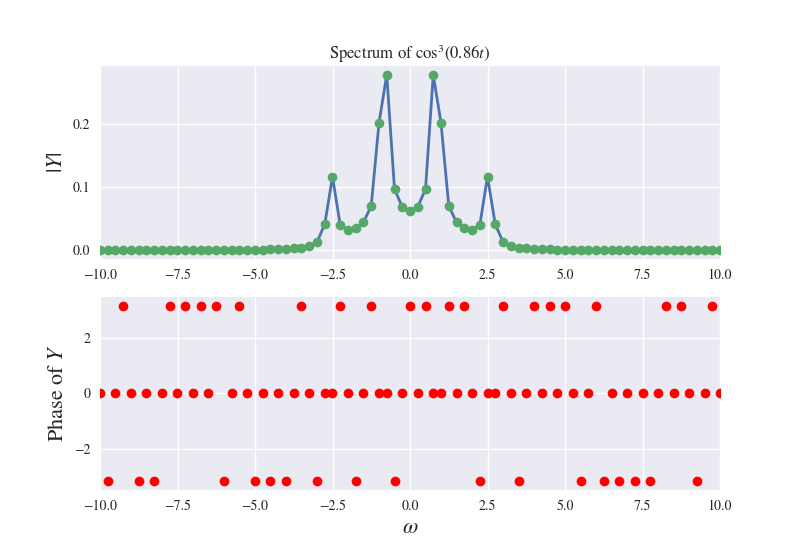
\includegraphics[scale=0.7]{images/fig9.png}
\end{center}
With Windowing:
\begin{center}
    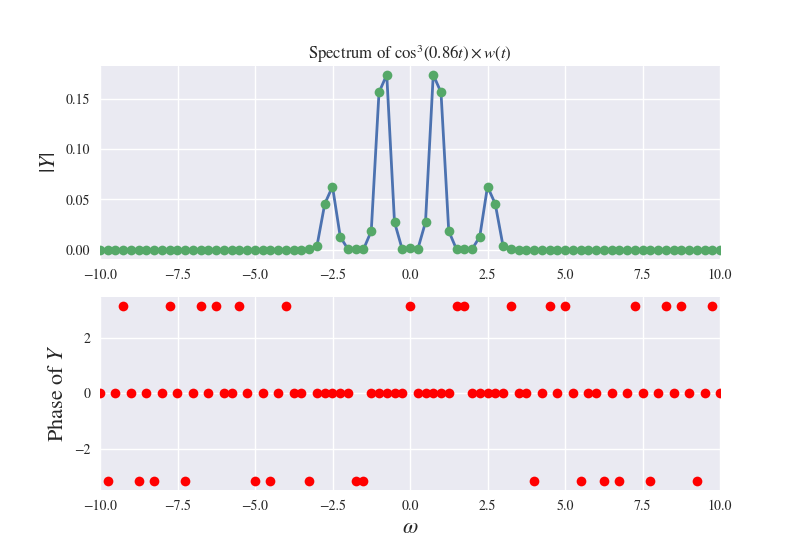
\includegraphics[scale=0.7]{images/fig10.png}
\end{center}
\pagebreak

\section{Question 3 - Estimation of $\omega$ and $\delta$ without noise}

For estimating $\omega$, we use the following formula:

$$\omega_0 = \frac{\sum |Y|^p omega}{\sum |Y|^p}$$

And the value of $\delta$ is nothing but the value of the angle at the argument for which the magnitude is maximized (i.e. where $\omega_0$ occurs).

The value of $p$ was chosen to be 1.7 after checking values from 1.0 to 3.0 in steps of 0.1, and this was found to be the closest value.

Function to Estimate $\omega$ and $\delta$:
\begin{lstlisting}[language=Python]
def om_del(func,ts,pow=1.7):
    N = len(ts)
    fmax = 1/(ts[1]-ts[0])
    w = np.linspace(-np.pi*fmax,np.pi*fmax,N+1)[:-1]
    y = func
    n = np.arange(N)
    wnd = fftshift(0.54+0.46*np.cos(2*np.pi*n/(N-1)))
    y = y*wnd
    y[0] = 0
    Y = np.fft.fftshift(np.fft.fft(np.fft.fftshift(y)))/N
    delta = np.angle(Y[::-1][np.argmax(abs(Y[::-1]))])
    omega = np.sum(abs(Y**pow*w))/np.sum(abs(Y)**pow)
    return omega,delta
\end{lstlisting}

Driver Code:
\begin{lstlisting}[language=Python]
omega = 0.5
delta = np.pi

# Now taking the fourier transform of cos(omega * t + delta)

t = np.linspace(-np.pi,np.pi,129)[:-1]
fmax = 1/(t[1]-t[0])
y1 = np.cos(omega*t + delta)
om,delt = om_del(y1,t,1.7)
print(f"The estimated value of omega is {om} and delta is {delt}")
\end{lstlisting}

\begin{center}
    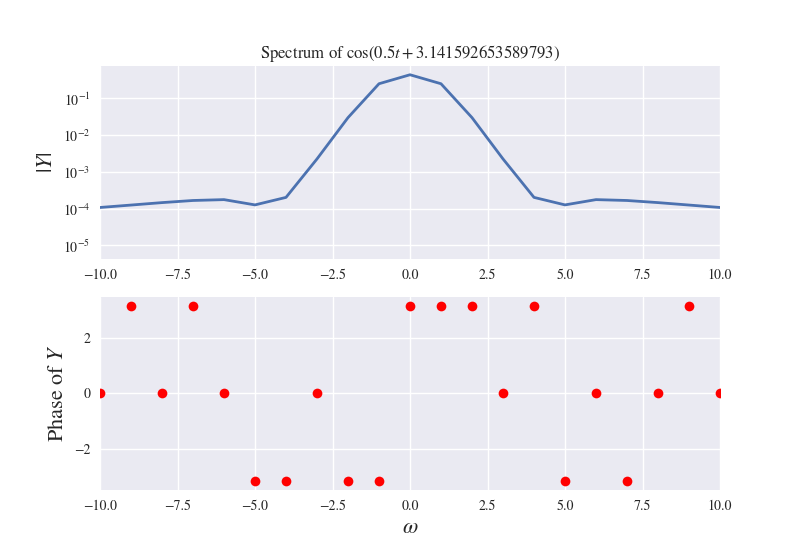
\includegraphics[scale=0.8]{images/fig11.png}
\end{center}

\subsection{Estimated Values}

The output is as follows:

\texttt{The estimated value of omega is 0.4512296880262127 and delta is 3.141592653589793}

Actual values were 0.5 and $\pi$, so the outcome is very close.

\pagebreak

\section{Question 4 - Estimation of $\omega$ and $\delta$ with White Gaussian noise}

Here too the function used is the same, but the value of $p$ is used as 2.4 instead of 1.7 as it is found to give the best accuracy upon testing values from 1.0 to 3.0 in steps of 0.1.

Driver Code:
\begin{lstlisting}[language=Python]
y2 = np.cos(omega*t + delta) + 0.1*np.random.randn(128)
om,delt = om_del(y2,t,2.4)
print(f"The estimated value of omega is {om} and delta is {delt}")

n = np.arange(128)
wnd = np.fft.fftshift(0.54+0.46*np.cos(2*np.pi*n/128))
y11 = wnd*y1
y11[0]=0
y11 = np.fft.fftshift(y11)
Y = np.fft.fftshift(np.fft.fft(y11))/128
w = np.linspace(-np.pi*fmax,np.pi*fmax,129)[:-1]
plot_spectrum(w,Y,ctr,rf"$\cos\left({omega}t+{delta}\right)$")
ctr+=1
plt.show()
\end{lstlisting}

\begin{center}
    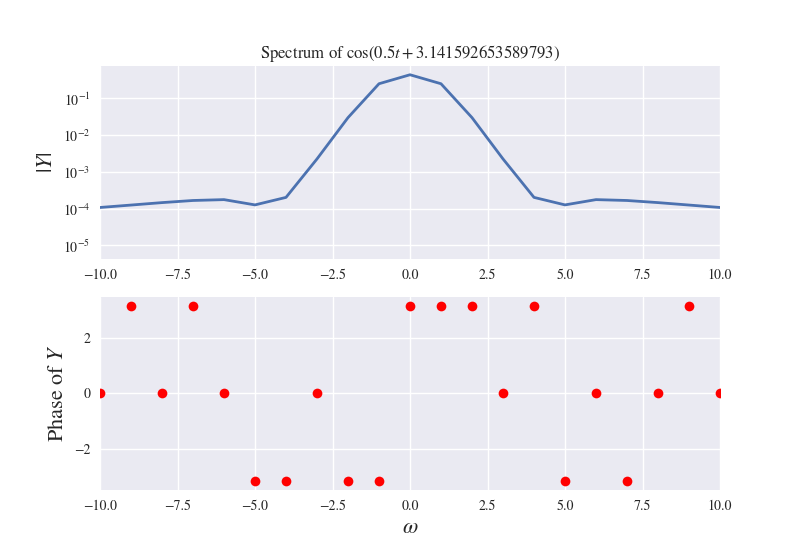
\includegraphics[scale=0.8]{images/fig11.png}
\end{center}


\subsection{Estimated Values}

The output is as follows:

\texttt{The estimated value of omega is 0.44844863425672743 and delta is 3.141592653589793}

The output is again close enough to the input values of 0.5 and $\pi$.
\pagebreak

\section{Question 5 - Chirped Signal}

This is a straightforward given input, and we plot the spectrum and the function.

\begin{lstlisting}[language=Python]
t = np.linspace(-np.pi,np.pi,1025)[:-1]
fmax = 1/(t[1]-t[0])
y = np.cos(16*t*(1.5+t/(2*np.pi)))
y = np.fft.fftshift(y)
Y = np.fft.fftshift(np.fft.fft(y))/1024
w = np.linspace(-np.pi*fmax,np.pi*fmax,1025)[:-1]
plot_spectrum(w,Y,ctr,r"$\cos\left(16t\left(1.5+\frac{t}{2\pi}\right)\right)$",type='linpts',xlims=[-50,50])
ctr+=1

y = np.cos(16*t*(1.5+t/(2*np.pi)))
plot_func([t], [y], ctr, r"$\cos\left(16t\left(1.5+\frac{t}{2\pi}\right)\right)$",save=True)
ctr+=1
\end{lstlisting}

Graphs obtained:
\begin{center}
    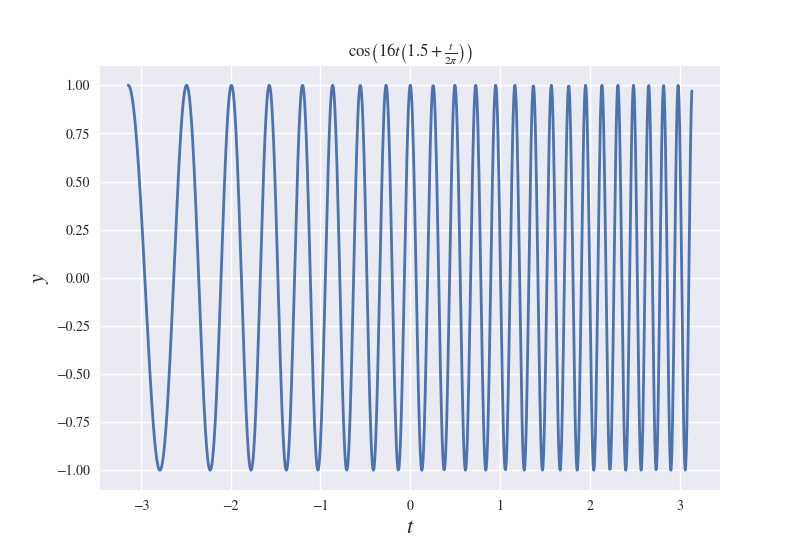
\includegraphics[scale=0.7]{images/fig13.png}
    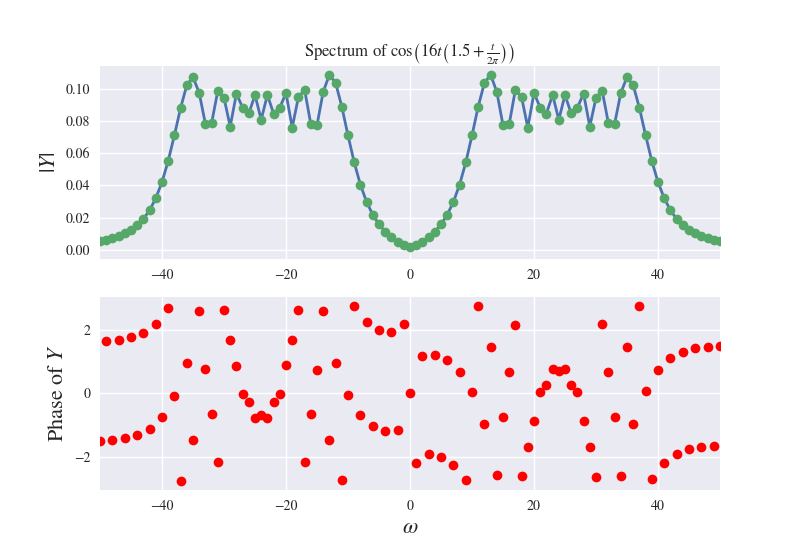
\includegraphics[scale=0.7]{images/fig12.png}
\end{center}

\pagebreak
\section{Question 6 - Chirped Signal Surface Plot}

We will be using a 3D plotting tool which is a part of matplotlib.

We will sample it over 16 different parts and plot them as a surface.

The code used is as follows:

\begin{lstlisting}[language=Python]
import mpl_toolkits.mplot3d.axes3d as ax3d

Ys = []
for i in range(16):
    tlow = np.pi*(-1+i/8)
    thigh = tlow+np.pi/8
    t = np.linspace(tlow,thigh,65)[:-1]
    y = np.fft.fftshift(np.cos(16*t*(1.5+t/(2*np.pi))))
    Y = np.fft.fftshift(np.fft.fft(y))/64
    Ys.append(Y)

Ys = np.asarray(Ys)
t1 = np.linspace(-np.pi,np.pi,16)
ts = np.linspace(-np.pi,np.pi,1025)[:-1]
fmax = 1/(ts[1]-ts[0])
w = np.linspace(-np.pi*fmax,np.pi*fmax,65)[:-1]
ax = ax3d.Axes3D(plt.figure(ctr))
ctr+=1
Ys1 = Ys.copy()
ii = np.where(abs(w)>150)
Ys1[:,ii]=np.NaN
t1,w = np.meshgrid(t1,w)
surface = ax.plot_surface(t1,w,abs(Ys1).T,rstride=1,cstride=1,cmap=plt.get_cmap("jet"))
plt.ylabel(r'$\omega\rightarrow$',size=16)
plt.xlabel(r'$t\rightarrow$',size=16)
ax.set_ylim([-150,150])
ax.set_zlabel(r'$|Y|$')
plt.show()
\end{lstlisting}
\pagebreak
The graphs obtained are as follows:

\begin{center}
    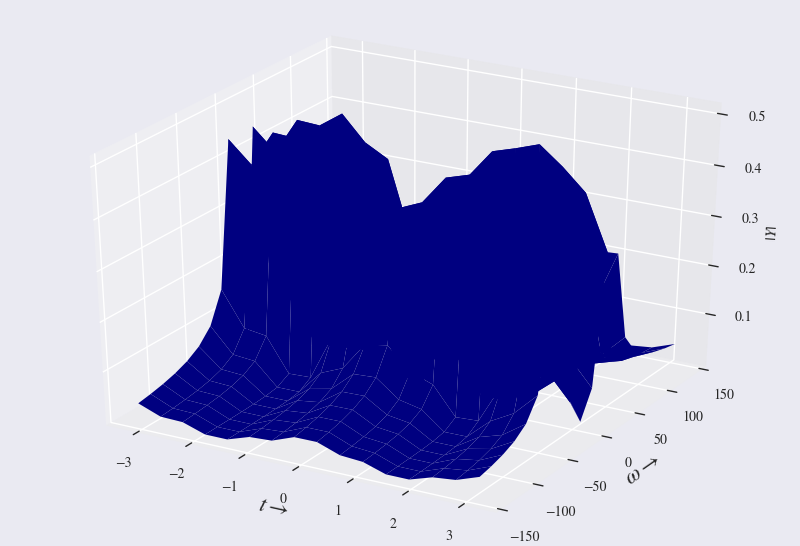
\includegraphics[scale=0.8]{images/fig14.png}
    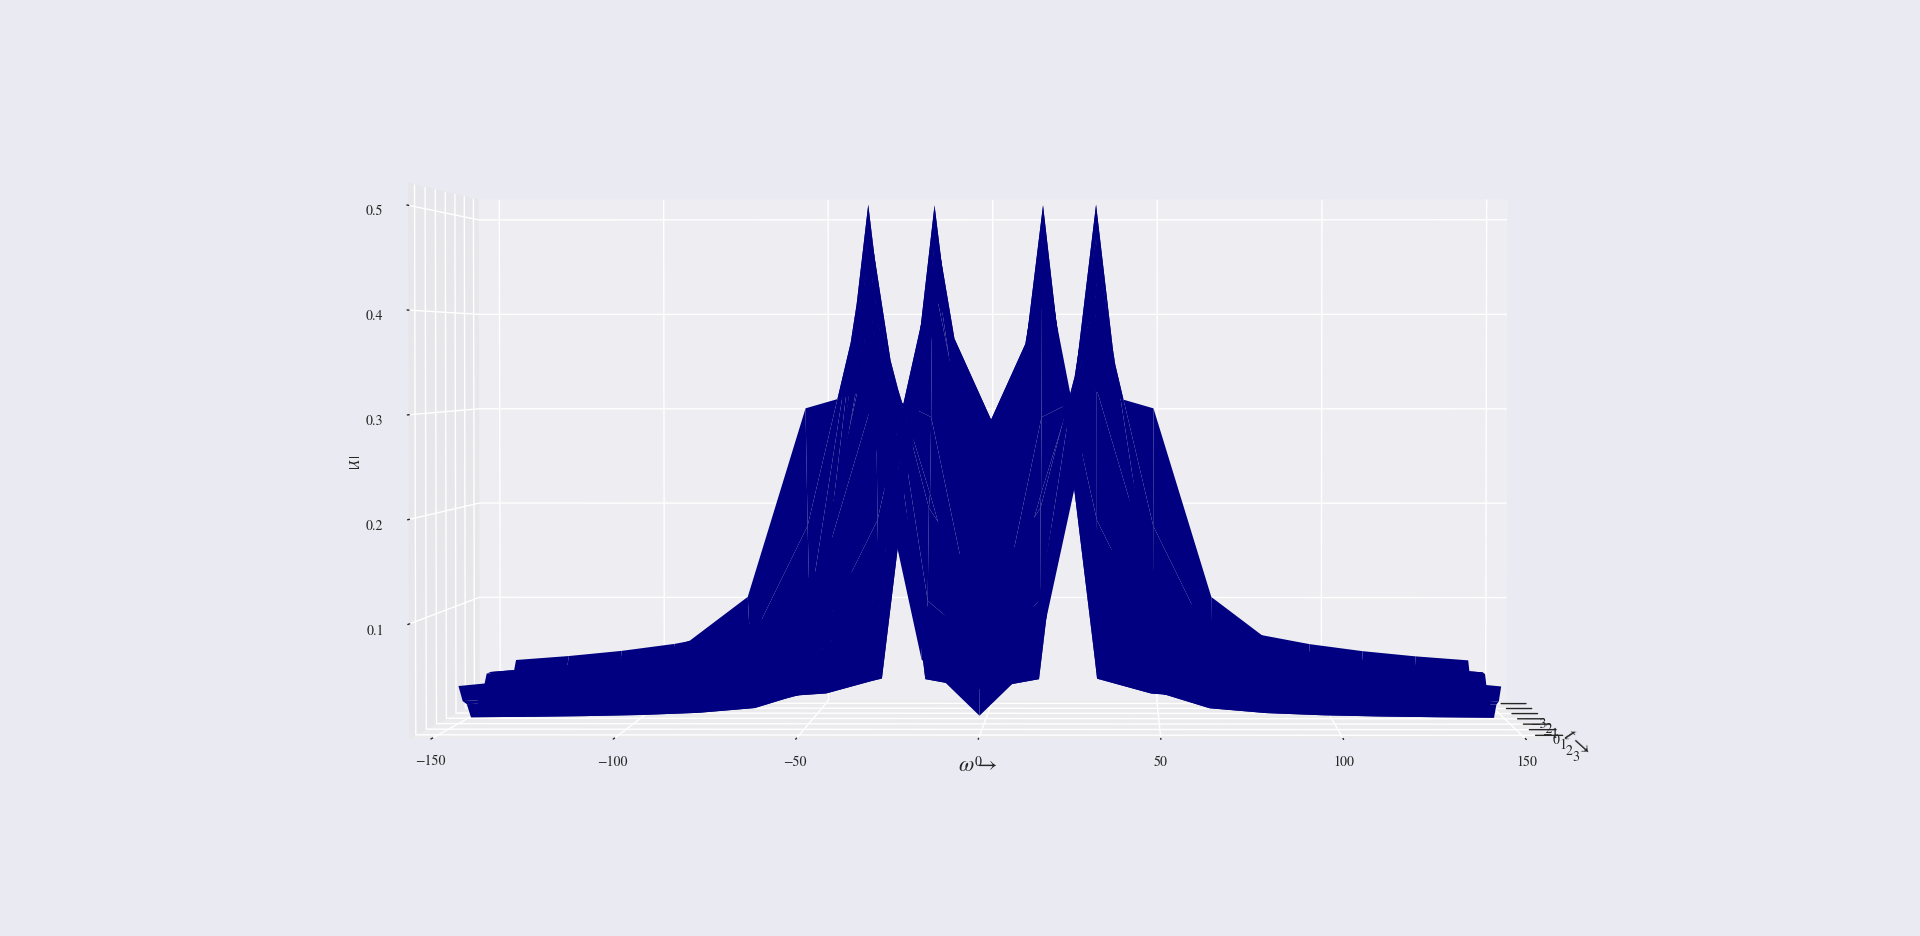
\includegraphics[scale=0.36]{images/fig14_1.png}
    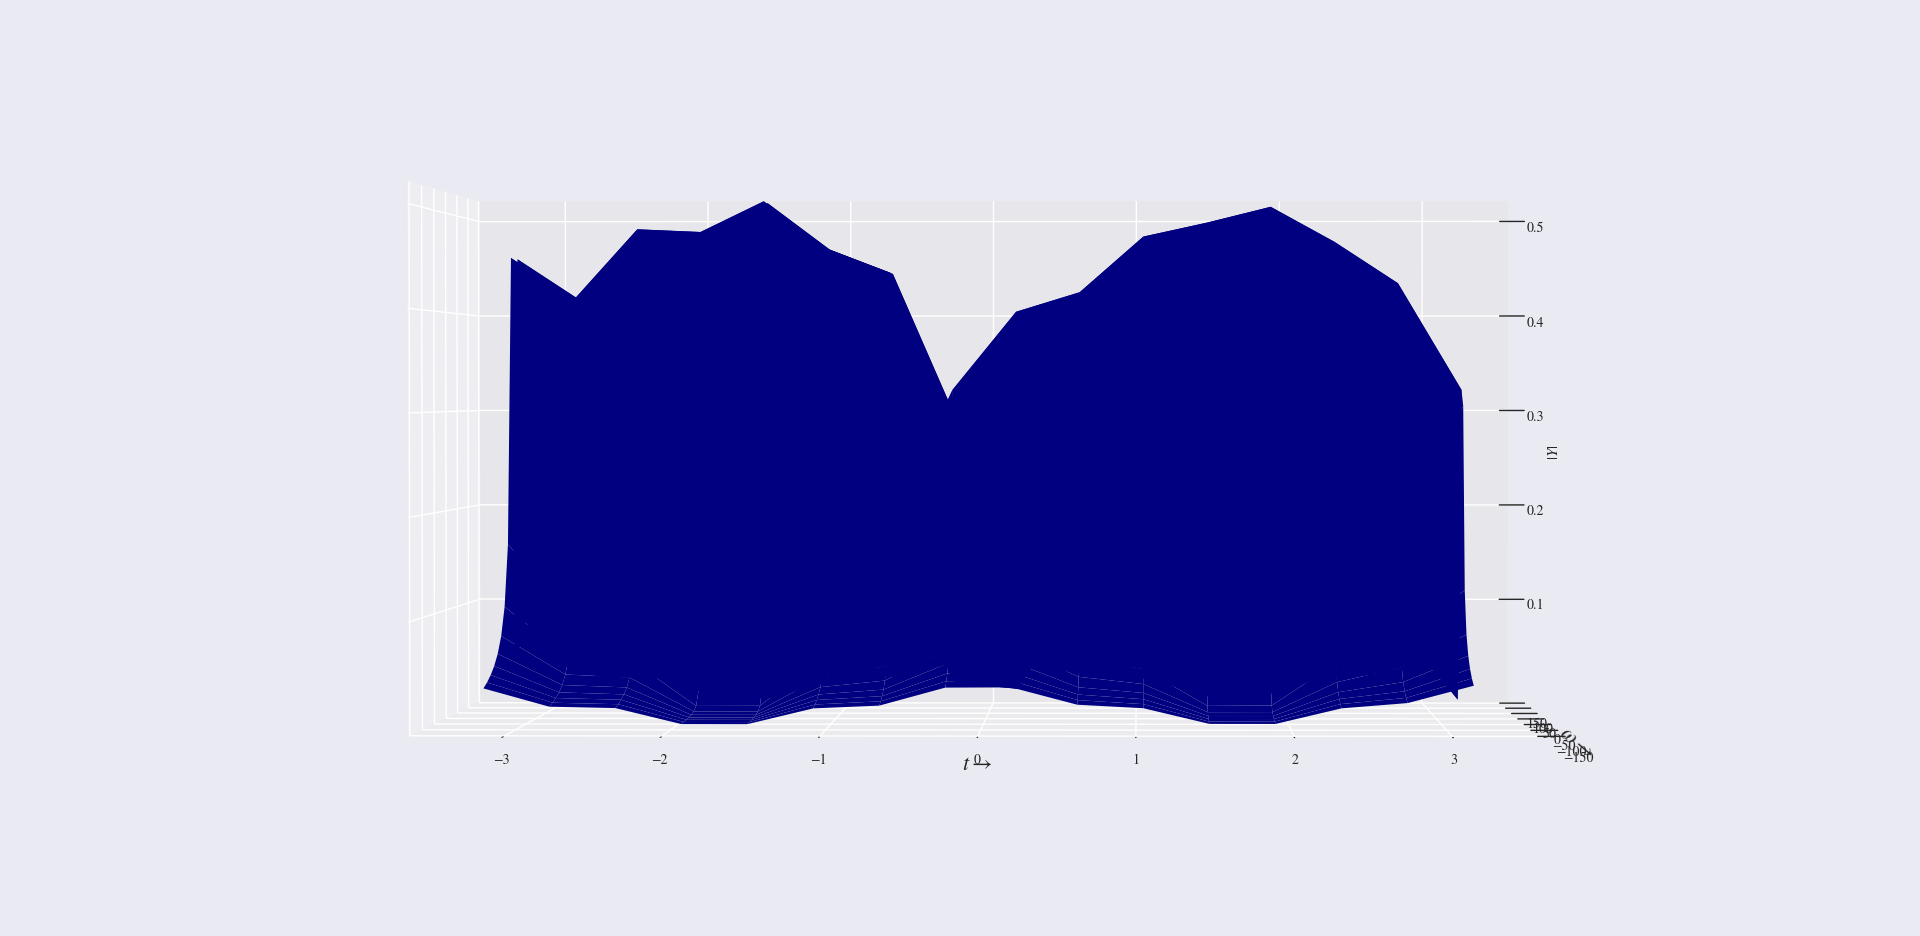
\includegraphics[scale=0.36]{images/fig14_1_2.png}
\end{center}

\section{Conclusions}

\begin{enumerate}
    \item Initially we had trouble getting the right spectrum as the DFT function was trying to use the $2\pi$ extension of a non-periodic function.
    \item This was resolved using the Hamming Window technique.
    \item Given cosine samples, the frequency and phase were calculated using an expectation value technique and argmax technique respectively.
    \item The DFT of a Chirped Signal was found to show a gradual variation of peak frequency with time and was symmetric in frequency.
\end{enumerate}

\end{document}
